\documentclass[11pt]{amsart}
\usepackage{geometry}                % See geometry.pdf to learn the layout options. There are lots.
\geometry{letterpaper}                   % ... or a4paper or a5paper or ... 
%\geometry{landscape}                % Activate for for rotated page geometry
%\usepackage[parfill]{parskip}    % Activate to begin paragraphs with an empty line rather than an indent
\usepackage{graphicx}
\usepackage{amssymb}
\usepackage{epstopdf}
\usepackage[usenames,dvipsnames]{color}
\usepackage{fancyvrb}
\usepackage{listings}
\usepackage{booktabs,footmisc}
\usepackage{hyperref}
\usepackage[all]{hypcap}

\usepackage{topcapt}


 
% include the lines below to use a nicer fixed-width font than the default one
 
\lstset{fancyvrb=true}
\lstset{
	basicstyle=\small\tt,
	identifierstyle=,
	commentstyle=\color{Bittersweet},
	stringstyle=\color{red},
	showstringspaces=false,
	tabsize=3,
	numbers=left,
	captionpos=b,
	xleftmargin=2em
%	numberstyle=\tiny
	%stepnumber=4
	}
\DeclareGraphicsRule{.tif}{png}{.png}{`convert #1 `dirname #1`/`basename #1 .tif`.png}

\title{Repast Statecharts Guide}
\author{Jonathan Ozik - Repast Development Team}
\date{\today}                                           % Activate to display a given date or no date

\begin{document} 
\maketitle
\setcounter{section}{-1}

\section{Before we Get Started}
Before we can do anything with Repast Simphony, we need to make sure that we have a proper installation of Repast Simphony 2.1. Instructions on downloading and installing Repast Simphony on various platforms can be found on the \href{http://repast.sourceforge.net/download.html}{Repast website}.

\section{Getting Started with Statecharts}

\section{States}
One of the fundamental building blocks of statecharts are states. Here we introduce the different types of states that existing within the Repast Simphony statecharts framework.

\subsection{Entry State Marker}

\includegraphics[height=.2in]{StatechartsImages/First-State-32.png}

Every statechart must have an entry state marker. This defines the path through which the statechart begins when it is activated.

\subsection{Simple State}
\label{sec:simpleState}

\includegraphics[height=.2in]{StatechartsImages/State-32.png}

A simple state looks like Figure~\ref{fig:simpleState}. At any one point in time within an active statechart, one and only one of the simple states will be active. In addition to their \emph{ID}, simple states can have \emph{On Enter} and \emph{On Exit} actions defined, as seen in the simple state properties panel in Figure~\ref{fig:simpleStateProperties}. These actions are triggered when entering or exiting the simple state, respectively. The keywords available within the action blocks are:
\begin{description}
\item[agent] This is the agent that contains the statechart. Any method (e.g., \texttt{customMethod}) defined on the agent can be invoked through this reference (e.g., \texttt{agent.customMethod()}).
\item[state] This is the state itself. The state's \emph{ID} can be accessed via: \texttt{state.getId()}.
\item[params] This is the model's \texttt{Parameters} object. As an example, a double valued parameter ``dParam" can be retrieved with: \texttt{params.getDouble("dParam")}\footnote{See the source or JavaDocs for  \texttt{repast.simphony.parameter.Parameters} for all of the available methods.}.
\end{description}

As is the case with all types of action blocks, the code within them can be defined using Java, Groovy or ReLogo. Any Java, Groovy or ReLogo code can be used to specify the type of behavior that should be executed upon entry to or exit from the state\footnote{When using the ReLogo option, the \texttt{agent} parameter is implicit so \texttt{customMethod()} is equivalent to \texttt{agent.customMethod()}.}.

\begin{figure}
\begin{center}
\vspace{.2in}
\centerline {
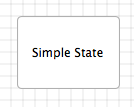
\includegraphics[width=1in]{StatechartsImages/SimpleState.png}
}
\caption{Simple state.}
\label{fig:simpleState}
\end{center}
\end{figure}

\begin{figure}
\begin{center}
\vspace{.2in}
\centerline {
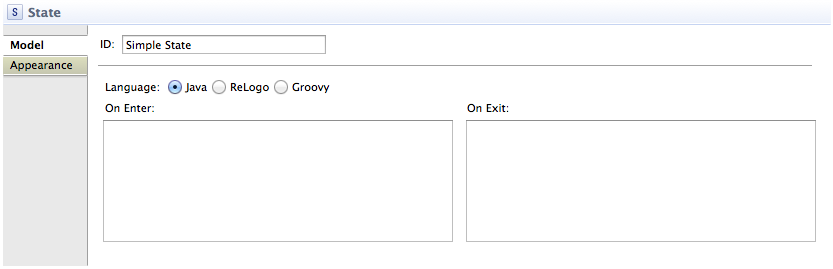
\includegraphics[width=5in]{StatechartsImages/SimpleStateProperties.png}
}
\caption{Simple state properties.}
\label{fig:simpleStateProperties}
\end{center}
\end{figure}

\clearpage

\subsection{Composite State}
\label{sec:compositeState}

\includegraphics[height=.2in]{StatechartsImages/Composite-State-32.png}

Composite states are used to nest elements within a statechart. Figure~\ref{fig:compositeState} shows an empty composite state. Composite states can include the following elements:
\begin{itemize}
\item Simple state (Section~\ref{sec:simpleState})
\item Composite state (Section~\ref{sec:compositeState})
\item Initial state marker (Section~\ref{sec:initialStateMarker})
\item History state (Section~\ref{sec:historyState})
\item Final state (Section~\ref{sec:finalState})
\item Branching state (Section~\ref{sec:branchingState})

\end{itemize}

\begin{figure}
\begin{center}
\vspace{.2in}
\centerline {
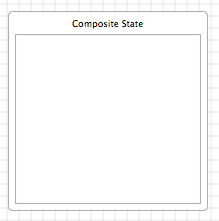
\includegraphics[width=2in]{StatechartsImages/CompositeState.png}
}
\caption{Composite state.}
\label{fig:compositeState}
\end{center}
\end{figure}

\begin{figure}
\begin{center}
\vspace{.2in}
\centerline {
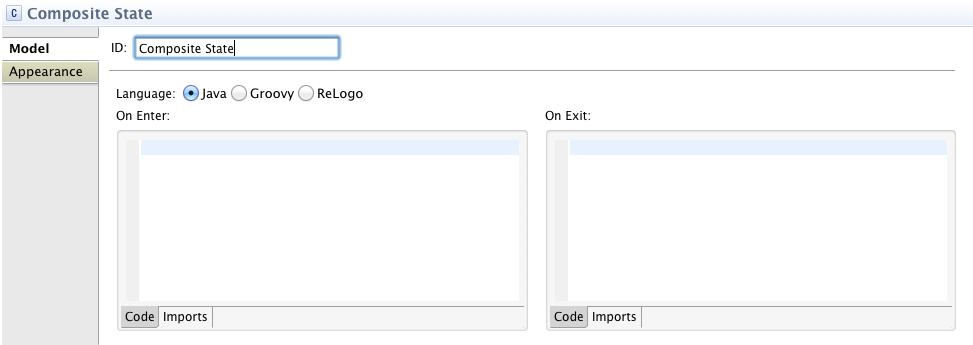
\includegraphics[width=5in]{StatechartsImages/CompositeStateProperties.png}
}
\caption{Composite state properties.}
\label{fig:compositeStateProperties}
\end{center}
\end{figure}

\clearpage

\subsection{Initial State Marker}
\label{sec:initialStateMarker}

\includegraphics[height=.2in]{StatechartsImages/Initial-State-32.png}

\begin{figure}
\begin{center}
\vspace{.2in}
\centerline {
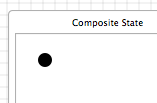
\includegraphics[width=1.5in]{StatechartsImages/InitialStateMarker.png}
}
\caption{Initial state marker (within a composite state).}
\label{fig:initialStateMarker}
\end{center}
\end{figure}


\subsection{History State}
\label{sec:historyState}

\includegraphics[height=.2in]{StatechartsImages/Shallow-History-32.png} 
\includegraphics[height=.2in]{StatechartsImages/Deep-History-32.png}

\subsection{Final State}
\label{sec:finalState}

\includegraphics[height=.2in]{StatechartsImages/Final-State-32.png}

\subsection{Branching State}
\label{sec:branchingState}

\includegraphics[height=.2in]{StatechartsImages/Choice-32.png}

\section{Transitions}
\subsection{Always Transition}
\subsection{Timed Transition}
\subsection{Probability Transition}
\subsection{Condition Transition}
\subsection{Exponential Decay Rate Transition}
\subsection{Message Transition}
\subsubsection{When Message Meets Condition}
\subsubsection{When Message Equals}
\subsubsection{When Message is of Class}
\subsubsection{Always}



\end{document}  